\section{Project Management}\label{project-sec}

\TODO{Shreyas Srinivas and Pietro Monticone have volunteered to take the lead on this section.}

This project is, among other things, an experiment on how to organise large scale collaborations for mathematical work. In this section, we describe several aspects of the mechanics of the collaborative effort.

\subsection{Problems of scale in mathematical collaboration}
In order to understand the difficulties of scaling that arise in large scale collaborations, it helps to revisit how traditional mathematical collaborations work and understand why they may not scale. Every collaboration is unique, and we cannot imagine that any universal template exists. However, some general patterns can be observed in any mathematical collaboration. Usually, a small number of contributors, usually under ten, who may know each other, join forces to tackle some class of problems. Typically the collaborators are academics who share substantial amounts of common knowledge. They discuss the problem at hand together, typically with some shared written medium such as a whiteboard. After several rounds of discussion and refinement, different members of the collaboration come up with different pieces of the solution and discuss how they fit together into a whole. Along the way, each collaborator writes out their specific contributions and reviews that of others. After several iterations of this process they synthesize the results into a single paper. At this point, the collaborators are reasonably confident about the correctness of their work, including theorem statements and proofs, and submit the paper for peer review. Of course, there are many variations to this general template, but the basic cycle of discuss, solve, write, cross-check, and revise process is always present in some form or another. Point 4 of the EMS code of practice for joint responsibility \cite{EMS_code_of_practice} explicitly specifies that the correctness of published work is the joint responsibility of all co authors.

However this project involved over fifty contributors spread across the world with diverse academic and professional backgrounds. They collaborated across several timezones and countries over the internet. The aforementioned process does not scale. Collaborators do not usually know each other nearly as well as they would in a traditional project. Further, as the number of contributors grows beyond the single digits, it becomes increasingly difficult to ensure that robustness of each other's results. Joint responsibility implies that all authors ought to understand and check theorems and proofs written by everybody else. Concretely, the scaling challenge manifests in several ways:
\begin{itemize}
    \item Partitioning and allocating tasks to voluntary contributors, keeping track of progress on the respective subtasks, and ensuring that everybody gets a fair chance at contributing without conflicting submissions for the same subproblems.
    \item Homogenising the content of discussions which could span multiple online conversation threads into a coherent outline of progress in a specific subproblem
    \item Tracking progress relative to the goals of the project on the number and list of remaining equational law pairs becomes almost impossible without automation.
    \item Verifying the correctness of contributions made by over fifty people with diverse backgrounds who might not share a common mathematical vocabulary, but happen to  collaborate across multiple timezones, using a diverse set of tools.
\end{itemize}

Of the challenges mentioned above, this section deals with the first, second, and last. We briefly address the third challenge of tracking progress, the tools for which are described in \Cref{sec:gui-sec}. We spend a lot of time on the last point of trust and verification of results for two reasons. On the one hand, use of tools like Lean is fairly new in mathematical research, and while the community researching theorem provers is familiar with their guarantees and limitations, a clear academic exposition targeted at mathematics researchers will be a helpful resource for future reference, to fill a gap that is currently covered by online forums and folklore.

\subsection{Organising the collaboration : The precedent set by the PFR project}
When five people collaborate in-person, splitting up the research on a question into subtasks and assigning them to collaborators can be accomplished by discussion and consensus. When there are more than fifty collaborators working together online, a more systematic approach is required. In previous formalisation projects such that the formalisation of the proof of the Polynomial Freiman Rusza conjecture \cite{PFR_Tao_Dilles_2023}, tasks were managed over the lean zulipchat forum. The maintainer of the project posted a series of message threads. Each thread corresponded to a list of outstanding tasks. These tasks were then claimed by collaborators on Zulip. The claims were recorded on a first come first serve basis by the maintainer by tagging the respective users against the tasks. Contributors could claim any open task and disclaim tasks if they couldn't finish it, with the maintainer keeping track of these requests. This system allowed contributors to take their time to flesh out their work, without worrying about their work being wasted by another collaborator unknowingly working on the task simultaneously. This is substantially different contributions models of open source projects which do not discourage competition among participants to accomplish the same goals. Further, it helped the maintainers track the task assignment and communicate with the respective collaborators to track and ascertain progress. Unfortunately, this involved a lot of manual and time-consuming management of the task list by maintainers. In this project, we took a different approach, several pieces of this approach were automated. This freed up maintainers to help contributors and review their contributions.

\subsection{Organizing the collaboration in this project:}
In this project, we very quickly reached the scalability limits of organising tasks solely via the Zulipchat forum. Instead we adopted tools that are familiar to software engineers as ticket systems but are also known in the wider world of industrial production, such as the eponymous kanban system that originated in the kanban cards used by Toyota to organise its production processes. We made use of the github project feature. In addition to the in-built task automation provided with github projects, we included additional automation through \emph{continuous integration} scripts (hereon CI). The exact flow of contributions is specified in the \emph{CONTRIBUTING.md} file of the project repository. Briefly,

\begin{enumerate}
    \item Tasks are proposed by maintainers. A contributor might start a discussion on Zulip or raise an issue on the github to prompt the maintainers to launch tasks.
    \item Contributors could then claim tasks with a comment under the task. The CI ensured that at most one contributor could claim a task at any time.
    \item Contributors could then work on the task and propose a corresponding pull request.
    \item Upon completion of the task, the pull request receives reviews, while the CI automatically checks that the project compiles and passes additional checks such as lean' environment replay tool \emph{leanchecker}.
    \item If all is well, the PR is merged onto the main branch of the project repository.
\end{enumerate}

At any point in this process, the contributor can disclaim the task or replace a proposed PR with an alternative. In addition, maintainers could always step in to fix any errors that occur and follow up with contributors. Each of the steps described above happened automatically, triggered by a well defined set of actions described in the \emph{CONTRIBUTING.md} file. The typical workflow of this process is shown in the flowchart in \Cref{fig:proj_mgmt_flow}. The figure omits error handling and situations where maintainers might manually intervene. The user interface to this project management is the github project dashboard, of which we include a snapshot in \Cref{fig:proj_dashboard}

\begin{figure}[t]
    \centering
    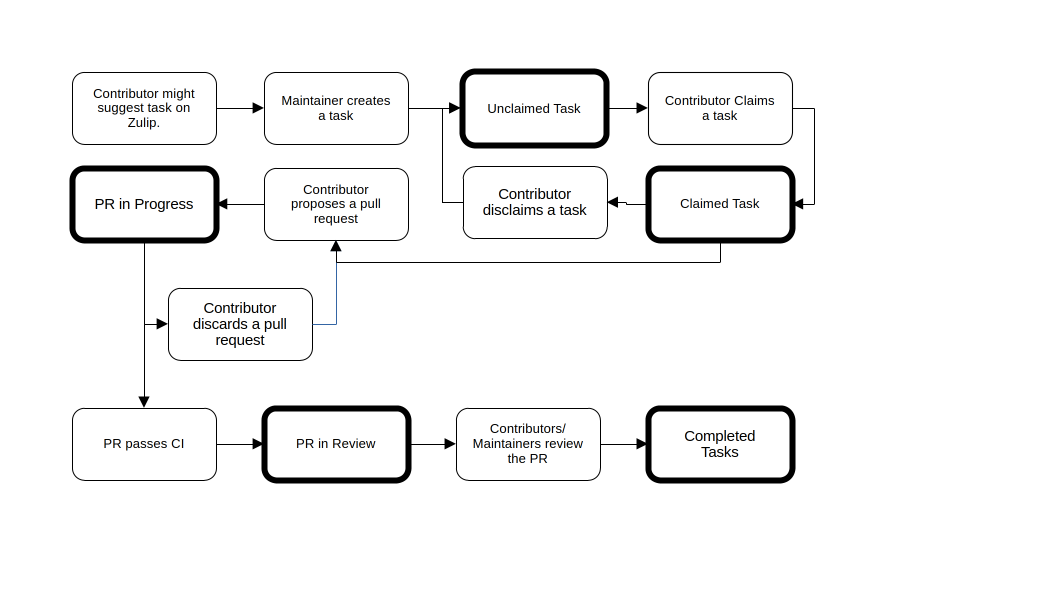
\includegraphics[width=1.0\textwidth]{proj_mgmt_figures/task_flowchart.png}
    \caption{\label{fig:proj_mgmt_flow} A partial flowchart of the automated task management process. Each task corresponds to an issue. A pull request is created to resolve tasks and once a pull request linked to a task is merged, the task is considered complete. The thick boxes represent states of the project dashboard represented by task columns. The movement of tasks between these states is automated by the CI which is triggered upon specific actions performed by contributors on the respective github issues and pull requests. A more detailed description is found in the contributions file of the github file, named CONTRIBUTING.md by convention.}
\end{figure}

\begin{figure}[t]
    \centering
    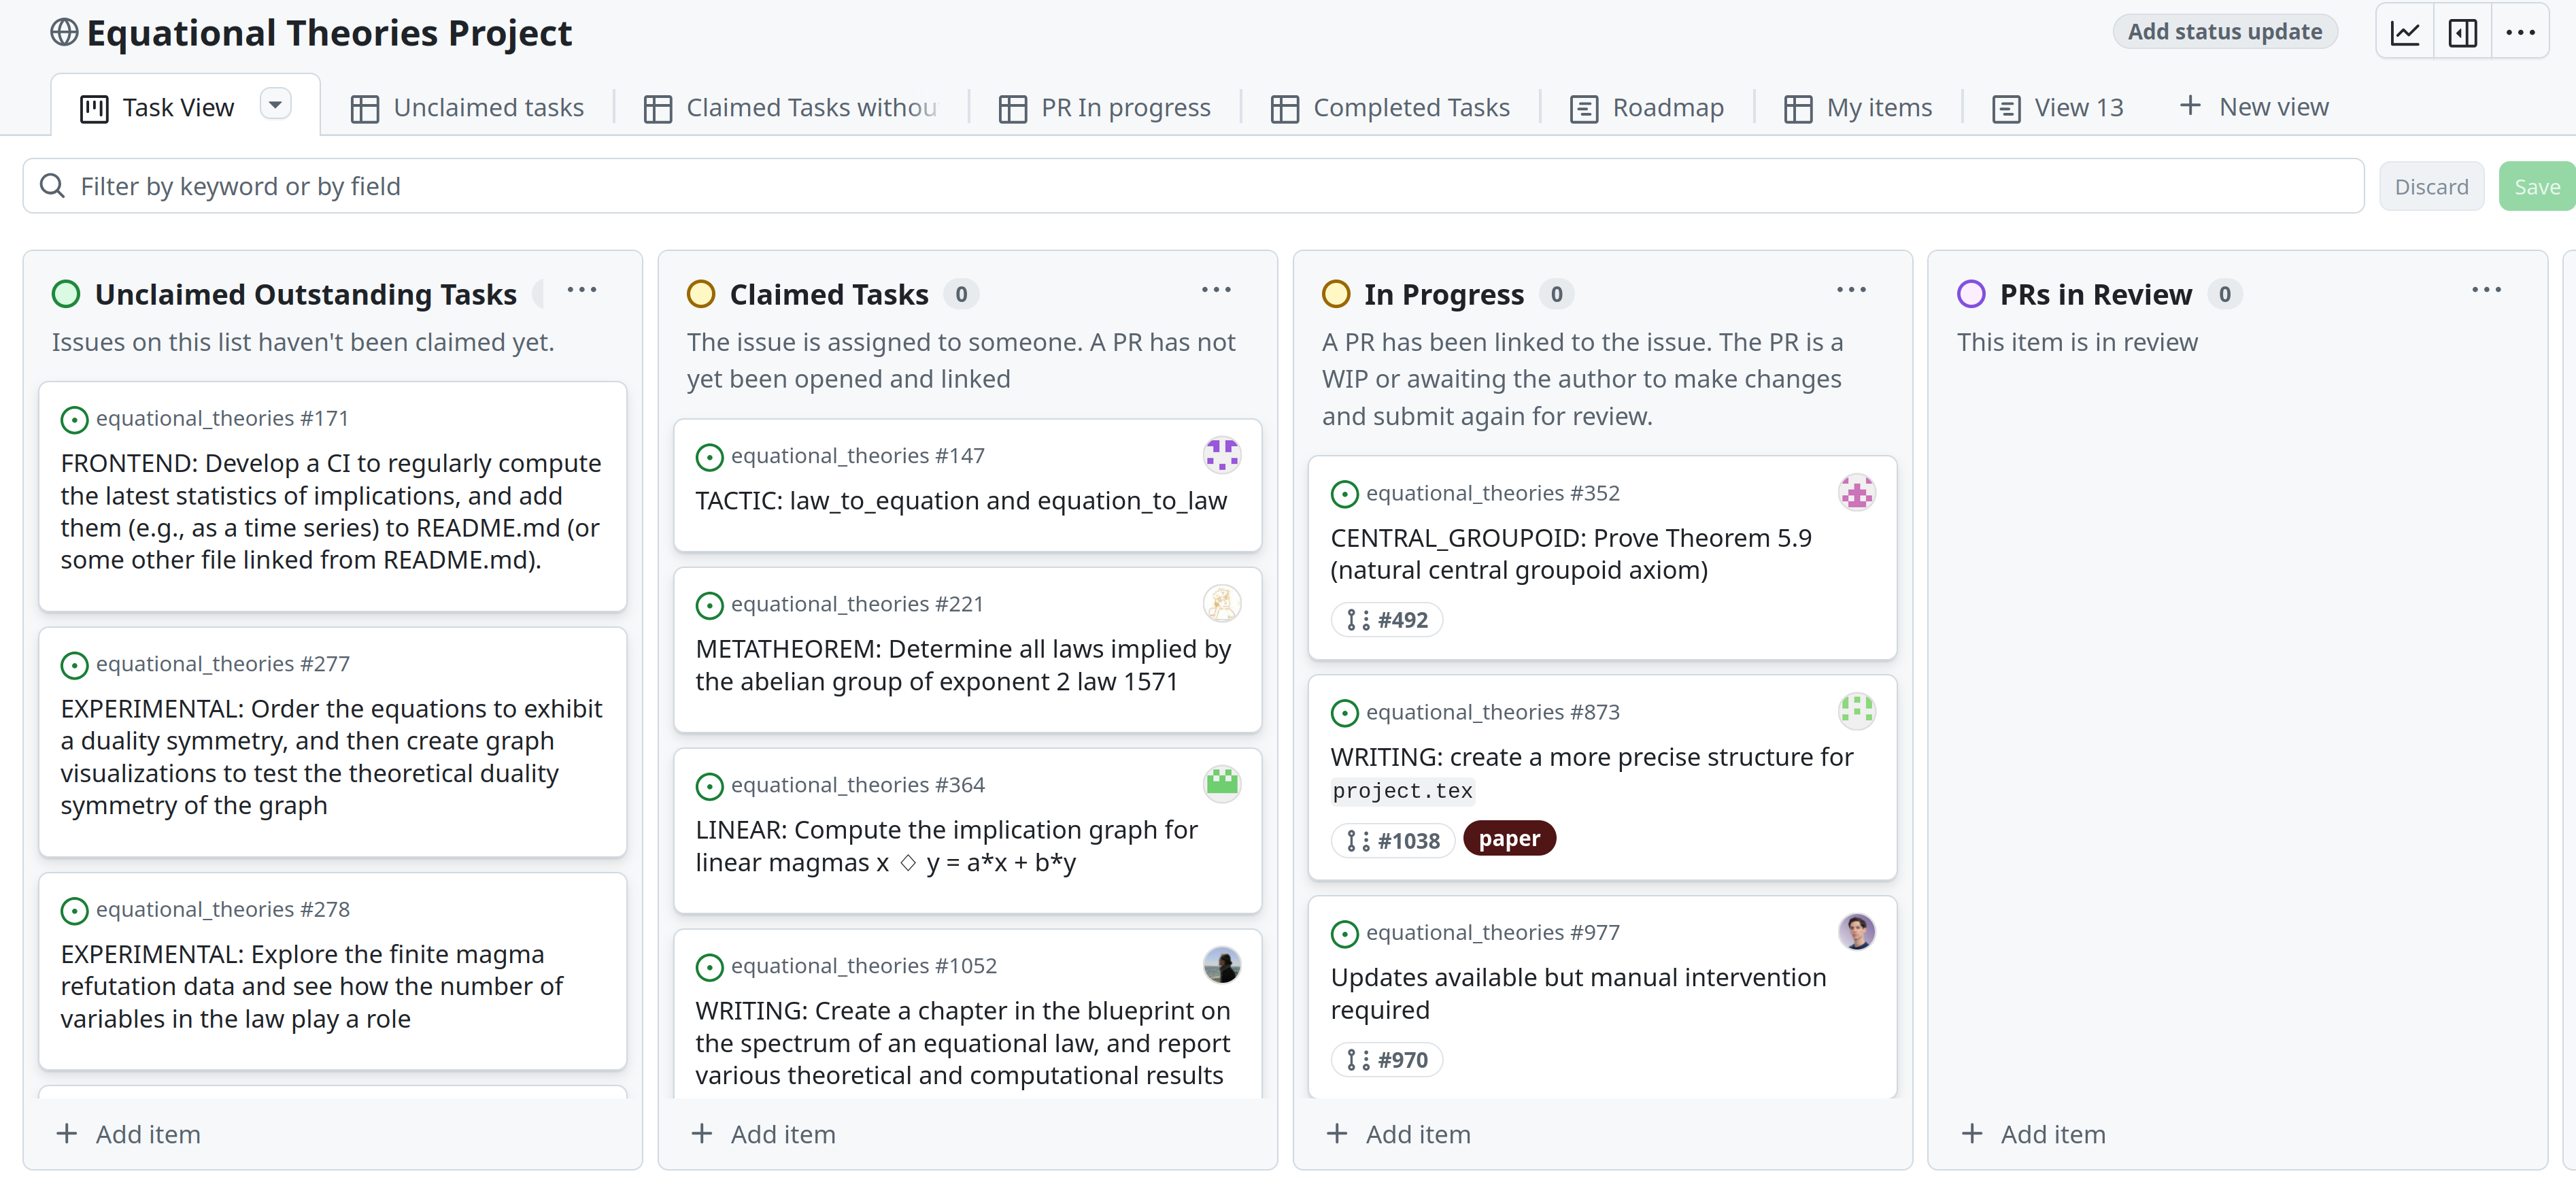
\includegraphics[width=1.0\textwidth]{proj_mgmt_figures/proj_dash_snapshot.png}
    \caption{\label{fig:proj_dashboard} A snapshot of the project dashboard as of July 30th 2025}
\end{figure}
\subsection{Trusting ITPs to Scale Collaboration}
In our project we used the interactive theorem prover lean 4 \cite{the_lean4_paper} precisely to address these issues of scaling.

At its core, an interactive theorem prover implements an expressive logic, encoded in a suitable choice of mathematical foundations. In particular Lean 4 has the calculus of constructions extended by inductive types as its core logic. This logic is sufficiently powerful to express mathematical definitions and theorems for almost all areas of mathematical interest. Additionally, modern ITPs provide a convenient programming language which helps express mathematical ideas in a syntax closer to a mathematician's intuition than would be permitted by raw logical terms. A subset of ITPs like Lean, Rocq (formerly Coq), and Isabelle go one step further and provide the means to generate proofs through so-called \emph{tactics}. There are usually numerous tactics, each specialised for specific kinds of proof generation, and their functionalities can include, for instance, searching mathematical libraries, simplification of expressions, resolution of propositional conundrums etc. The basic idea is that the proofs generated by this overlying programming machinery are checked mechanically by a spartan proof checker. But in a large project, trust is a complicated business, even with Lean. It helps to understand the nature and limits of trust one can place on ITPs. The project management issues described in this section exist precisely to navigate around these limitations and deliver on the promise of large scale collaboration that ITPs offer.

It helps to understand exactly what it means to trust lean. As mentioned before, conceptually, lean consists of two pieces:

\begin{enumerate}
    \item A core proof checker called the \emph{kernel}. This checker encodes a typed $\lambda$-calculus that is sufficiently expressive for most mathematical purposes. Without getting into details, theorems are encoded as a formal specification of the intended theorem statement. Proofs are encoded as deduction trees using known lemmata, acceptable axioms, and inference rules. The kernel checks whether this deduction tree constitutes a correct deduction in the context of existing theorems and lemmata, called the \emph{environment}. Once a theorem's proof has been checked, it is added to the environment and can be used for constructing subsequent proofs.
    \item A sophisticated programming language in which users express their definitions and theorems. Programs in this language are said to  be \emph{elaborated} to produce definitions and proofs in the core logic that the kernel can check.
\end{enumerate}

Of these two pieces, \emph{only the kernel is considered trusted}. Programs in the programming language are translated by an \emph{elaborator} to the spartan language of the kernel. In reality the elaborator does much more, but the key takeaways from this is the following:
\begin{itemize}
    \item The kernel only verifies programs of a very simple barebones language. A proof verified by Lean can be trusted \emph{modulo} the correctness of the kernel implementation. This caveat can be usually dropped because, the kernel is also one of the most battle-hardened pieces of an ITP.
    \item The kernel checks proofs against a given specification. This means that if the formal theorem statement itself is flawed or incorrectly uses other definitions, a correct and verified proof of this theorem would be mathematically meaningless. The formal statement of a theorem gives expression to a mathematician's intuition and intention, and as such, the only check against mistakes in this area come from human review. Lean cannot offer any guarantees against false statements written by its users.
    \item The higher level programming language can in-principle, generate arbitrary deductions. Their correctness is ultimately validated by the kernel. This gives the higher level programming language more leeway in generating arbitrary deductions.
    \item Ideally the environment only consists of lemmata already checked by the kernel. Thus their correct usage in the proof of subsequent theorems is valid. However this assumption can be bent in practical implementations of theorem provers for efficiency reasons. In this case, trust in the kernel is restored by replaying each assumption from scratch in the kernel. This can be accomplished by external checkers. Such checkers, which are ideally independent implementations of the \emph{kernel}, can also guard against implementation mistakes in the kernel.
\end{itemize}

\begin{remark}
    A bug in the kernel that allows wrong statements to be proved is usually called a \emph{soundness} bug. Concretely this means that a proof of the vacuous proposition $False$ can be produced and pass the kernel check. Such bugs are rare but not entirely non-existent \TODO{Collect a couple of example github issues/tickets of soundness bugs across ITPs}. This is distinct from being able to proof $False$ by simply assuming contradictory or false statements. A proof of the proposition $False$ implies a proof of any statement by the emph{ex falso quod libet} inference rule.

\end{remark}

Users of lean only interact directly with the higher level programming language and usually get confirmation of the correctness of their proofs through the editor interface. Further, collaborators on a project such as ours are likely to deploy automated tools such as SAT solvers, SMT solvers, first-order theorem provers, and perhaps even modern AI tools. These tools usually produce proofs which are imported or inserted into a lean source files. Some modern AI tools are integrated into code editors which might automatically produce or edit even the statements of theorems and the definitions they deal with. Given the limits to trust mentioned above, a productive and useful collaboration using lean also requires a collaboration and verification infrastructure which involves both human effort and automated tools. It is in this context that we discuss the project infrastructure. It is a concrete answer to the questions posed by one of the authors at the beginning of this project \cite{Tao_blog_Sep_2024} that combines tools from the ITP community and the software engineering community. All these tools are known well in these fields.The goal of this exposition is to explain how they allay the concerns described above.

\TODO{This would be a good point to describe the role of maintainers and reviewing. It would also serve to explain how the external checkers integrate with the CI. Maybe we can blend it all into what has been written so far}
\begin{itemize}
    \item Project generation from \href{https://github.com/pitmonticone/LeanProject}{template}
    \item GitHub issue management with \href{https://github.com/teorth/equational_theories/labels}{labels} and \href{https://github.com/users/teorth/projects/1}{task management dashboard}
    \item Continuous integration (builds, blueprint compilation, task status transition)
    \item Pre-push git hooks
    \item Use of blueprint (small note, see \#406: blueprint chapters should be given names for stable URLs)
    \item Use of Lean Zulip (e.g. use of polls)
\end{itemize}

Maybe give some usage statistics, e.g. drawing from \url{https://github.com/teorth/equational_theories/actions/metrics/usage}

Mention that FLT is also using a similar workflow.

\subsection{Handling Scaling Issues}

Also mention some early human-managed efforts ("outstanding tasks", manually generated Hasse diagram, etc.) which suffices for the first one or two days of the project but rapidly became unable to handle the scale of the project.

Mention that some forethought in setting up a GitHub organizational structure with explicit admin roles etc. may have had some advantages if we had done so in the planning stages of the project, but it was workable without this structure (the main issue is that a single person -- Terry -- had to be the one to perform various technical admin actions).

Use of transitive reduction etc.\ to keep the Lean codebase manageable. Note that the project is large enough that one cannot simply accept arbitrary amounts of Lean code into the codebase, as this could make compilation times explode. Also note somewhere that transitive completion can be viewed as directed graph completion on a doubled graph consisting of laws and their formal negations.

Technical debt issues, e.g., complications stemming from an early decision to make Equations.lean and AllEquations.lean the ground truth of equations for other analysis and visualization tools, leading to the need to refactor when AllEquations.lean had to be split up for performance reasons.

Note that the "blueprint" that is now standard for guiding proof formalization projects is a bit too slow to keep up with this sort of project that is oriented instead about proving new results. Often new results are stated and formalized without passing through the blueprint, which is then either updated after the fact, or not at all. So the blueprint is more of an optional auxiliary guiding tool than an essential component of the workflow.

\subsection{Other Design Considerations}

Explain what "trusting" Lean really means in a large project. Highlight the kind of human issues that can interfere with this and how use of tools like external checkers and PR reviews by people maintaining the projects still matters. Provide guidelines on good practices (such as branch protection or watching out for spurious modifications in PRs, for example to the CI). Highlight the importance of following a proper process for discussing and accepting new tasks, avoiding overlaps etc. These issues are less likely to arise in projects with one clearly defined decision maker as in this case, and more likely to arise when the decision making has to be delegated to many maintainers.

Note that despite the guarantees provided by Lean, non-Lean components still contained bugs. For instance, an off-by-one error in an ATP run created a large number of spurious conjectures, and some early implementations of duality reductions (external to Lean) were similarly buggy. "Unit tests", e.g., checking conjectured outputs against Lean-validated outputs, or by theoretical results such as duality symmetry, were helpful, and the Equation Explorer visualization tool also helped human collaborators detect bugs.

Meta: documenting thoughts for the future record is quite valuable. It would be extremely tedious to try to reconstruct real-time impressions long after the fact just from the GitHub commit history and Zulip chat archive.

\subsection{Maintenance}

Describe the role of maintainers and explain why they need to be conversant in the mathematics being formalised, as well as Lean. As such, the role of maintainers is often akin to postdocs or assistant profs in a research group who do some research of their own, but spend much of their time to guide others in performing their tasks, the key difference being that contributors are volunteers who choose their own tasks. Explain the tasks maintainers must perform. Examples:

\begin{itemize}
    \item Reviewing proofs,
    \item Helping with proofs and theorem statements when people get stuck,
    \item Offering suggestions and guidance on how to produce shorter or more elegant proofs,
    \item Ensuring some basic standards are met in proof blocks that make proofs robust to upstream changes,
    \item Creating and maintaining CI processes,
    \item Responding to task requests,
    \item Evaluating theorem and definition formulations (for example unifying many theorem statements into one using FactsSyntax),
    \item Suggesting better ones where possible,
    \item Ensuring that there is no excessive and pointless overlap of content in different contributions \TODO{elaborate on what level of overlap was permissible and what we consider excessive}.
\end{itemize}
